\chapter*{INTRODUCTION}
\addcontentsline{toc}{chapter}{INTRODUCTION}
\addcontentsline{toc}{section}{General overview and motivations}
\noindent
\emph{Helicopter's vibrations} is a long-standing problem. Since the earliest days of rotor-craft development, oscillatory motion of the non-rotating portion of the airframe has been a matter of serious concern, from several viewpoints. \\ In fact, one of the reasons is that typically \emph{oscillatory motions} mean \emph{oscillatory strains} and oscillatory strains often involve \emph{fatigue of structural components} which affect the service life, increase the maintenance costs, reduce the availability of the machine and the safety of the flight itself. \\
Similarly, vibrations constitute a problem for equipments of all kinds; they make instruments hard to read, sight hard to aim and the add to fatigue of pilots, crew and passengers. \\

\noindent For these and many other reasons, vibration is an unwanted phenomenon in rotor-craft's design and operations and must be seriously faced by engineers since the beginning. \\
Unfortunately, helicopters are really complex machines with many rotating components and so they are intrinsically subject to vibrations which must be reduced or damped. \\

\medskip
\begin{figure}[h]
	\begin{center}
		\centering  		 		
		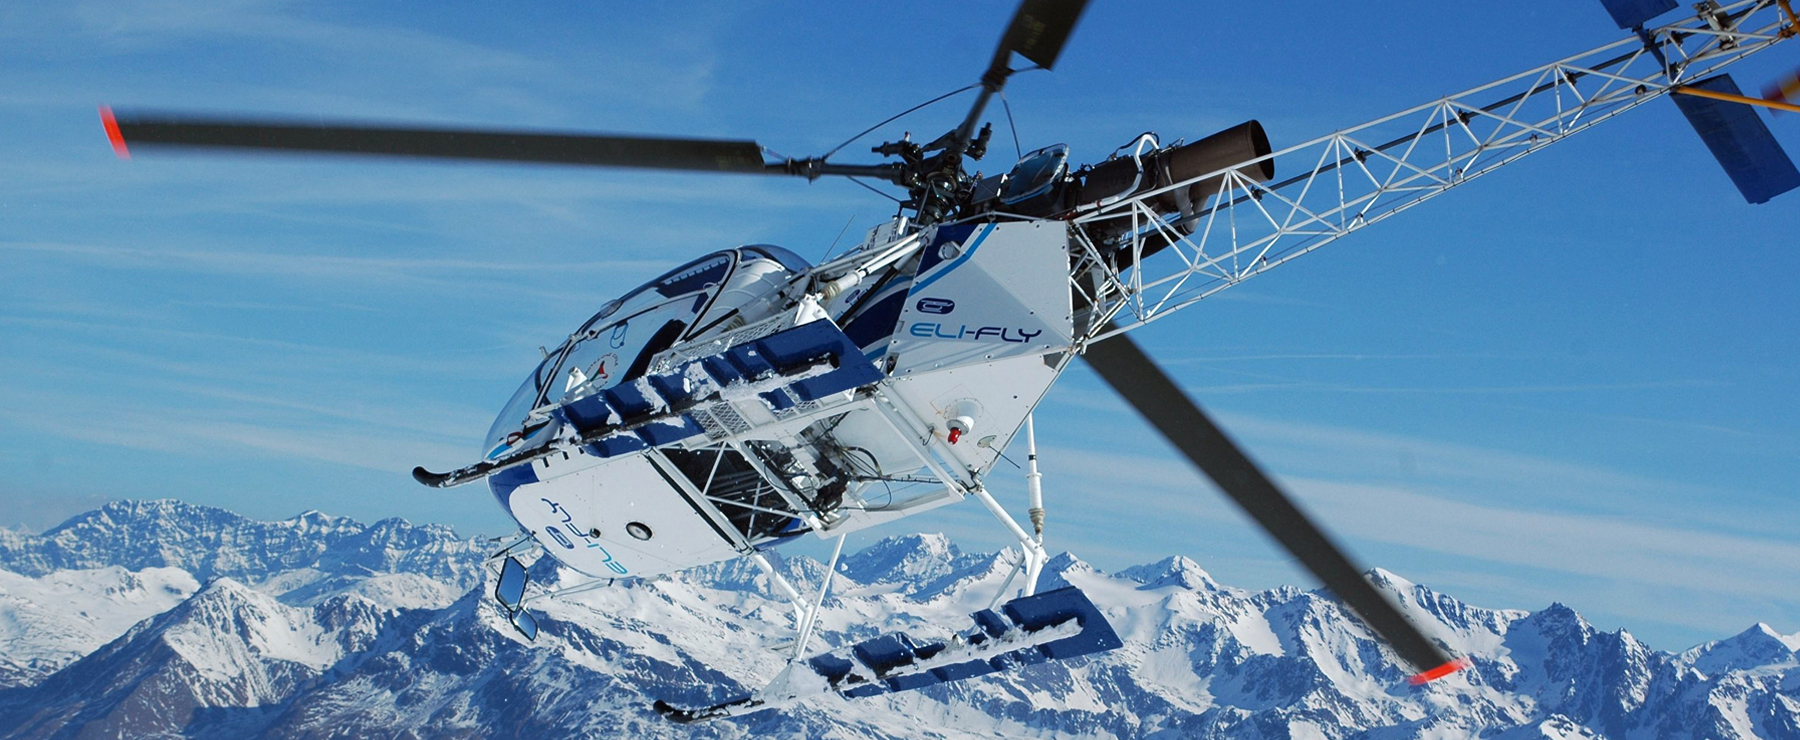
\includegraphics[width=1\linewidth]{PICTURES/Introduction/PNG/Elicottero_montagne.jpg}
	\end{center}
	\caption {A turbine helicopter during an in-flight manoeuvre}
\end{figure}
\vspace{0.5cm}

\noindent
There are many \underline{sources of vibration excitation} in a helicopter: for example,
\begin{itemize}
	\item engine and gearbox vibratory forces;
	\item main and tail-rotor excitations;
	\item rotor-mass imbalance;
	\item inertial and centrifugal accelerations due to manoeuvres during the flight. 
\end{itemize}

\bigskip
\noindent
Although the tail rotor causes a lesser effect then the main rotor on the overall vibration of the helicopter, its effects cannot be neglected especially because \emph{airframe vibrations are also typically amplified cause of the lightweight and flexible fuselage design}. \\
The primary causes of rotating machinery vibration are unbalances, misalignments, looseness and the excitation of structural resonances by rotating shaft running frequencies and their harmonics. Other sources of vibration can be bearing defects, insufficient lubrication and dirt entrapment between moving or rotating surfaces. \\
Excessive vibration of tail rotor can cause the tail section of helicopters to be physically ripped from the main structural assembly, and result in catastrophe. Severe imbalance in the rotating parts also can lead to instabilities during flight. \\

\noindent
Unfortunately, \underline{the complete helicopter vibration problem is virtually impossible to predict} \underline{accurately}, as yet, because of its structural, as well as aerodynamic, complexity. \\
To make the helicopter vibration problem more tractable, \emph{simplifying assumptions} must be made, especially for the rotor-dynamics analysis. Typically, the rotor system and the fuselage are analyzed separately and then attempts are made to account for rotor-fuselage coupling.
However, this procedure is questionable because it does not account for rotor-fuselage coupling. 
Even introducing an equivalent rotor mass, although it gives a somewhat better approximation, still does not adequately represent the coupled rotor-fuselage system. Thus, there appears to be no viable alternative to carrying out a coupled rotor-fuselage analysis when one is investigating fuselage response to rotor excitation. \\

\noindent
In the past, the vibration had not been considered in design phase of a helicopter, but nowadays, in order to minimize the costs and increase the comfort on-board, the vibration is being taken into account at design
stage. \\ With this aim, \emph{\underline{there is a need to evaluate the vibration primarily obtaining a model of the} \underline{structure as accurate as possible} including all the secondary structures and subsystems in the model as well as considering the coupling between the fuselage and the rotor}. \\ This is the way we intended to approach the problem. \\


\clearpage
\subsection*{Project's goals}
\addcontentsline{toc}{section}{Project's goals}

\noindent
In order to develop an improved understanding of the tailboom and rotor vibration characteristics of a helicopter, this research project was undertaken with the following main objectives : 
\begin{itemize}
	
	\item Present the problem and its importance that has recently gained in the design and manufacturing operations of the rotor-craft companies; 
	
	\item analyze the free helicopters tailboom's vibrations developing accurate Finite Element Models of the two simplified types of tailboom structures;
	
	\item improve the models accuracy taking into account also the presence of additional subsystems
	normally fixed on helicopter's tail but neglecting, at this step, the tailrotor movement (\emph{uncoupled tailrotor-fuselage dynamic models});
	
	\item improve the understanding of the techniques and phenomena regarding the \emph{tailrotor-fuselage dynamic coupling} which considers also the interaction and the effects related to the the tail-rotor rotation presenting 3 possible ways to approach the problem;
	
	\item explore the recently implemented Ansys Rotor-dynamic capabilities and	tools building a simplified rotor model to study the rotor's vibrational behaviour which results to vary with tail rotor speed.
\end{itemize}

\bigskip